\pagebreak
\subsection{Development environment}

Since the project should be developed for more than one mobile platform, it is important to make a good choice between different development environments and frameworks. The focus of this project will be on Android operating system, although application will be ported and developed for both iOS and Android.
As so, most convenient environments seem to be Eclipse and NetBeans.\newline

Eclipse is a multi-language software development environment comprising an integrated development environment (IDE) and an extensible plug-in system. It is written mostly in Java and can be used to develop applications in Java and, by means of various plug-ins, other programming languages, such as Android. 
To set it up and running, it is necessary to have Java Development Kit – JDK installed. Also, Android SDK must be downloaded, and with a custom plugin for the Eclipse, called Android Development Tools (ADT), integrated environment is set up to build and test Android applications.\newline

As already mentioned, PhoneGap will be used to develop and deploy project onto multiple platforms.\newline
\begin{figure}[phonegap]
	\centering
	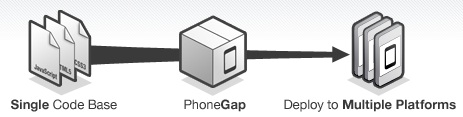
\includegraphics[width=0.8\textwidth]{prestudy/development_environment/PhoneGap.jpg}
	\caption{Multiple platforms deploying}
	\label{fig:phonegap}
\end{figure}
